\chapter{Einleitung}

In den vergrangenen Jahren hat \ac{KI} in Unternehmen zunehmend an Bedeutung gewonnen. Seit 2019 verzeichnet der KI-Software Markt einen hohes Wachstum. Es wird davon ausgegangen, dass dieses Wachstum bis 2025 mit über 26 \% pro Jahr anhalten wird. \footcites[Vgl.][]{howarth_57_2024} Die Anwendungsbereiche von KI-Systemen sind vielfältig und reichen von der Automatisierung von Prozessen, über die Analyse von großen Datenmengen bis hin zur Vorhersage von zukünftigen Ereignissen.

Einer der beliebtesten Anwendungsbereiche von KI-Systemen ist die Dokumentenverarbeitung. Eine Befragung von 1420 IT-Fachkräften ergab, dass 28 \% der zugehörigen Unternehmen KI-Systeme zur Dokumentenverarbeitung einsetzen (s. Abb. \ref{fig:ai_tech_distribution}). \footcites[Vgl.][]{rackspace_most_2023} Die Dokumentenverarbeitung umfasst die Extraktion von Informationen, die Klassifizierung und die automatisierte Verarbeitung von Dokumenten.\footcites[Vgl.][S.1]{esposito_intelligent_2005} Die Verarbeitung von Dokumenten ist in vielen Unternehmen ein zeitaufwändiger Prozess, der durch den Einsatz von KI-Systemen automatisiert und beschleunigt werden kann.\footcites[Vgl.][S.11]{dutt_now_2024}

\pgfplotsset{compat=1.17} % Use the version of pgfplots you have installed

\begin{figure}[htb]
    \centering
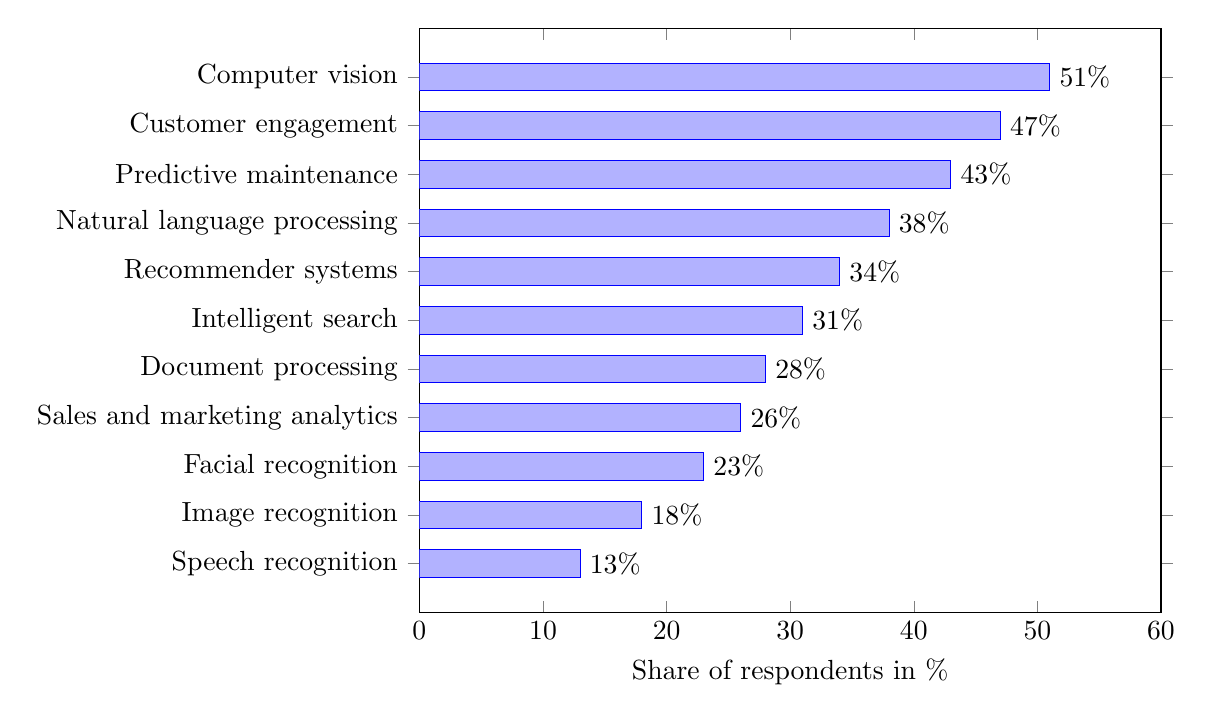
\begin{tikzpicture}
    \begin{axis}[
        xbar, % Horizontal bars
        xmin=0, xmax=60, % Set the minimum and maximum x-coordinates
        width=11cm, height=9cm, % Width and height of the plot
        enlarge y limits=0.1, % Add some space between bars
        xlabel={Share of respondents in \%}, % Label for the x-axis
        symbolic y coords={
            Speech recognition,
            Image recognition,
            Facial recognition,
            Sales and marketing analytics,
            Document processing,
            Intelligent search,
            Recommender systems,
            Natural language processing,
            Predictive maintenance,
            Customer engagement,
            Computer vision
        },
        ytick=data, % Use the data for y-ticks
        nodes near coords,
        nodes near coords align={anchor=west}, % Add the percentage labels near the bars% Align the labels horizontally
        point meta=explicit symbolic % The meta data is explicitly given as symbolic text
    ]
    \addplot [draw=blue,fill=blue!30 ] coordinates {
        (51,Computer vision)[51\%]
        (47,Customer engagement)[47\%]
        (43,Predictive maintenance)[43\%]
        (38,Natural language processing)[38\%]
        (34,Recommender systems)[34\%]
        (31,Intelligent search)[31\%]
        (28,Document processing)[28\%]
        (26,Sales and marketing analytics)[26\%]
        (23,Facial recognition)[23\%]
        (18,Image recognition)[18\%]
        (13,Speech recognition)[13\%]};
    \end{axis}
\end{tikzpicture}
\caption[Gängigste Verwendungszwecke von KI in Unternehmen]{Gängigsten Verwendungszwecke von KI in Unternehmen\footnotemark} % Caption for the figure
    \label{fig:ai_tech_distribution} % Label for referencing the figure
\end{figure}
\footnotetext{Entnommen aus: \cite{rackspace_most_2023}}

Die Verarbeitung von gescannten Dokumenten, insbesondere von Rechnungen ist ein integraler Bestandteil der Dokumentenverarbeitung. Der Einsatz von \ac{OCR} ermöglicht die Digitalisierung und elektronische Weiterverarbeitung dieser Dokumente. Jeoch ist die Zuordnung der erkannten Zeichenketten zu interpretierbaren Metadaten oft von manueller Nachbearbeitung oder von regulären Ausdrücken abhängig. Eine weitere Hürde, welche sich bei der Extraktion von Informationen aus Rechnungen zeigt, sind die sehr heterogenen Vorlagen und Layouts, welche in der Verarbeitung zu Ungenauigkeiten führen kann. Die OCR kann hier nicht mehr sicher die erkannten Werte den entsprechenden Labeln zuordnen.\footcites[Vgl.][S.1]{rahal_information_2018} Die DMS-Software \ac{ELO} von ELO verarbeitet Rechnungen zurzeit mittels OCR. Die Anwendung von Transformer-Modellen, im Bereich des \ac{VDU} ermöglicht eine direkte kontextbasierte Weiterverarbeitung der Rechnungen.\footcites[Vgl.][S.1]{kim_ocr-free_2021}

Diese Arbeit untersucht neue Transformer-Modelle im Bereich des VDU. Es wird analysiert, wie diese Modelle, die ihren Ursprng in der natürlichen Sprachverarbeitung haben, auf die Interpretation visueller (layoutbasierter) und textueller Elemente in Dokumenten angewandt werden können. Weiterhin wird ein OCR-freier \ac{Donut} untersucht, um die Limitierungen von OCR bezüglich Laufzeit und Fehleranfälligkeit zu überwinden.\footcites[Vgl.][S.1]{kim_ocr-free_2021} Diese Arbeit umfasst die Bereitstellung einer Pipeline, welche vom Modelltraining des Donuts bis zur Endanwendung im Unternehmen ELO Digital Office GmbH reicht. 
Das Ziel dieser Arbeit ist es, die Anwendbarkeit von Transformer-Modellen im Bereich des \ac{VDU} zu untersuchen und die Leistungsfähigkeit der Pipeline zu evaluieren um folgende Forschungsfrage zu beantworten:
\begin{center}
    \emph{Kann die Anwendung von Document Understanding Transformer Modellen die Effizienz und Genauigkeit der Rechnungsverarbeitung im Vergleich zu bestehenden OCR-basierten Modellen steigern?}
\end{center} 
Um diese Frage zu beantworten wird anhand eines Benchmarks (detaillierte Beschreibung des Aufbaus folgt in Kapitel 3) die Leistungsfähigkeit der Donut-basierten Pipeline mittels diverser Metriken bemessen und zur Leistungsfähigkeit von OCR-basierten Modellen verglichen. Daher ist die Arbeit folgedermaßen strukturiert: \\Zunächst werden in Kapitel 2 die Grundlagen der Dokumentenverarbeitung und der Transformer-Modelle erläutert. In Kapitel 3 werden die zu untersuchenden Modelle ausgewählt. Des weiteren werden der experimentelle Ansatz und der Aufbau der Testumgebung und Datensätze beschrieben. In Kapitel 4 wird die Entwicklung der Pipeline und die Implementierung des Donut dargestellt. Kapitel 5 präsentiert die Ergebnisse des Experiments. Kapitel 6 diskutiert die Ergebnisse und zieht Schlussfolgerungen. Eine Zusammenfassung und ein Ausblick auf zukünftige Arbeiten schließen die Arbeit in Kapitel 7 ab. Mit dieser Strukturierung als Ausgangspunkt, folgt nun die detaillierte Betrachtung der Grundlagen der Dokumentenverarbeitung und der Transformer-Modelle in Kapitel 2.
